% This is LLNCS.DEM the demonstration file of
% the LaTeX macro package from Springer-Verlag
% for Lecture Notes in Computer Science,
% version 2.4 for LaTeX2e as of 16. April 2010
%
\documentclass{llncs}
%
\usepackage{makeidx}  % allows for indexgeneration
% 
\usepackage{calc}
\usepackage{amssymb}
\usepackage{amstext}
\usepackage{amsmath}
\usepackage{color, colortbl}

\usepackage[final,pdftex]{graphicx}
        \pdfcompresslevel=9
        \DeclareGraphicsExtensions{.png} 

\usepackage{chngcntr}
\usepackage{epsfig} 
\usepackage{url}
 
\usepackage{ifthen} 
\usepackage{amssymb}
 
\usepackage{float} 
\begin{document}
%
\frontmatter          % for the preliminaries

\mainmatter              % start of the contributions
%
\title{EARS-CTRL: The Demonstration}
%
\titlerunning{}  % abbreviated title (for running head)
%                                     also used for the TOC unless
%                                     \toctitle is used
%
\author{Levi L\'ucio\inst{1} \and Salman Rahman\inst{1}
 \and Saad Bin Abid\inst{1} \and Alistair Mavin\inst{2}}
%
\authorrunning{} % abbreviated author list (for running head)
%
%%%% list of authors for the TOC (use if author list has to be modified)
\tocauthor{}
%
\institute{
fortiss GmbH\\
Guerickestra\ss e 25, 80805 M\"unchen\\
\email{\{lucio,abid\}@fortiss.org, salman.rahman@tum.de}\\
\and
Rolls-Royce, PO Box 31, Derby, UK\\
\email{alistair.mavin@rolls-royce.com}
}

\maketitle              % typeset the title of the contribution

\begin{abstract}
In this part of the paper, we demonstrate our tool in practice with the example
case study of a sliding door controller. We build controller specification in
natural language, automatically generate the controller and then perform
verification of the generated controller by utilizing testing and simulation
techniques. The demo video can be found at:
[URL: youtubevideo]
\end{abstract}

\vspace{-1cm}
\section{Introduction}
\label{sec:intro}
\vspace{-.4cm}
In this demonstration, we focus on providing a guidence to the users of our
tool. Our EARS-CTRL tool is a github project \cite{EARSProject}.
An overview of the demonstration steps is as follows,
\begin{itemize}
  \item Progressively build a set of requirements for the controller written in
  english like sentences using EARS lanaguage \cite{EARS}
  \item Automatic realisation of the controller by
  analyzing if the specification is complete (our one click approach)
  \item Simulation and test cases for performing conformance analysis between
  the EARS-based specification and the generated controller.
\end{itemize}
\vspace{-.5cm}
\section{The Running Example: Quiz Controller}
\label{sec:example}
\vspace{-.3cm}
Our running example for this demo is a Quiz Controller (QC) system
controller. The behavior of the sliding door controller is illustrated as a set
of \textsf{EARS-CTRL} requirements for the software controller for a QC as shown in
figure~\ref{fig:QC_reqs}.
\begin{figure*}[!h]
\centering
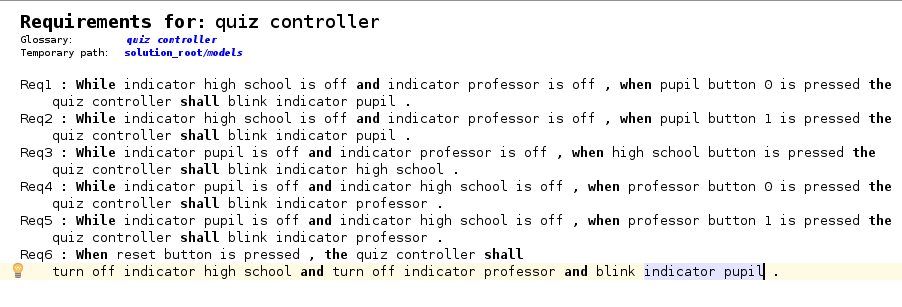
\includegraphics[width=1\textwidth]{./images/QC_Reqs.png}
\caption{Requirements written in \emph{EARS-CTRL} for a Quiz Controller}
\label{fig:QC_reqs}
\end{figure*}
\vspace{-.2cm}
\section{Tool Demonstration}
\label{sec:demo}
\subsection{Building a Glossary}
\vspace{-.1cm}
The first step towards writing the controller specifications in natural
language using \textsf{EARS-CTRL} is to define a glossary of terms. 
As is depicted in figure~\ref{fig:glossary_def}, the user is provided with an
editor to define glossary terms for: components that interface
with the controller; sensors and actuators those components make
available to the controller; invariant relations that should hold
between the sensor and actuator signals; and for ease of writing,
aliases to formulas involving sensors or actuators. During the demonstration we
will start from a glossary that is mostly built and will add the missing
components.
 
\vspace{-.2cm}
\begin{figure*}[!h]
\centering
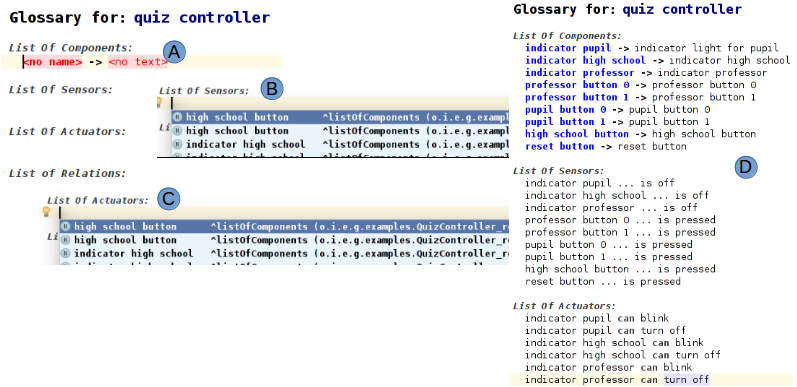
\includegraphics[width=1\textwidth]{./images/QC_Glossary_Def.png}
\caption{Step-by-step glossary building for a Quiz Controller: \emph{(A)}
components definition, \emph{(B)} sensors definition, \emph{(C)} actuators
definition and \emph{(D)} completed QC glossary}
\vspace{-.8cm}
\label{fig:glossary_def}
\end{figure*}
\subsection{Building \textsf{EARS-CTRL} requirements for the Quiz Controller}
\vspace{-.2cm}
Figure~\ref{fig:EARS_req} provides the set of steps required to write a set of
EARS requirements. In the projectional editor the user presses the CTRL+Space
key combination to instantiate an EARS-based template that presents a number of
placeholders (A). After obtaining an instance of the EARS template, the user
fills in the placeholders with information coming from the glossary definitions
(B). (C) depicts the complete Quiz Controller specification. As for the
glossary, during the demo we will use a mostly complete set of requirements and
will add the missing ones.
\begin{figure*}[!h]
\centering
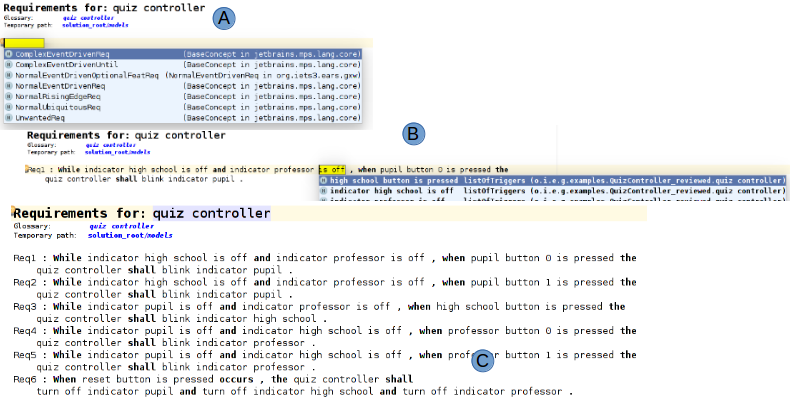
\includegraphics[width=1.2\textwidth]{./images/Req_Spec_Steps.png}
\caption{Step-by-step guidance for building controller requirements in
\textsf{EARS-CTRL}, (\emph{A}) empty instance of EARS template with placeholders, (\emph{B}) filling instance
of an EARS template with information and (\emph{C}) completed EARS Specification}
\label{fig:EARS_req}
\vspace{-.4cm}
\end{figure*}
\vspace{-.4cm}
\subsection{Synthesizing \textsf{EARS-CTRL} requirements}
\label{SynthReq}
\vspace{-.1cm}
Once the requirements for controller are completely specified, we will
synthesize the controller. For that the \emph{Transform} intention is used
by using the \emph{Alt+Enter} keys on the root of the specification (as shown in
(A) of figure~\ref{fig:Spec_transform}). The generated output after applying the
intention is comprised of: (B) the \emph{Synchronized Data Flow} (SDF) diagram
containing blocks connected by wires; (C) pseudo code representing the behavior
of each of the blocks used by the synthesized controller; (D) a Simulink block
diagram; and (E) empty panel for simulation and test case generation.
%\vspace{-.7cm}
\begin{figure*}[!h]
\centering
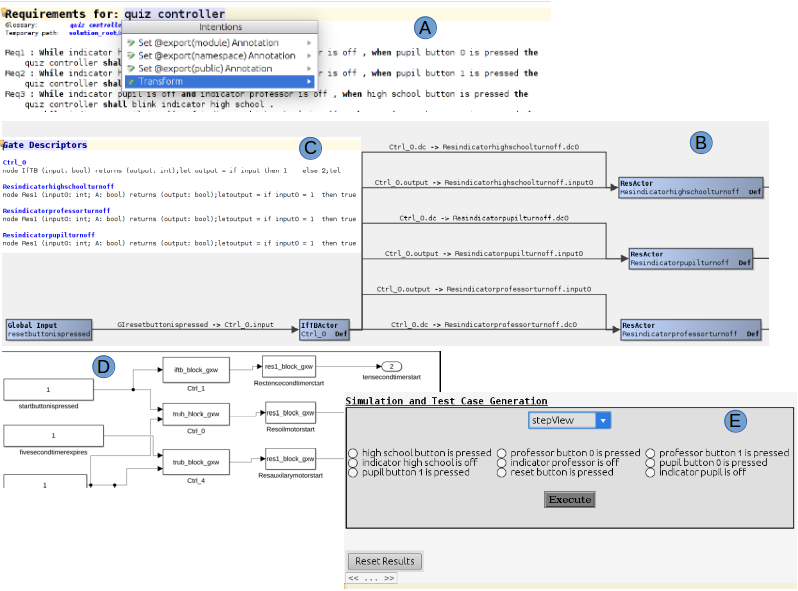
\includegraphics[width=1\textwidth]{./images/Transform.png}
\caption{Controller generation steps: (\emph{A}) applying intention \emph{Alt+Enter},
(\emph{B}) synchronized DFD of the controller (an excerpt), (\emph{C}) pseudo
code representing the behavior of the blocks (an excerpt), (\emph{D})
generated Simulink model (an excerpt) and (\emph{E})
generated empty panel for simulation}
\label{fig:Spec_transform}
\end{figure*}
\vspace{-.2cm}
\subsection{Simulation and Test Cases for Validation of Controller
Behavior}
\vspace{-.1cm}
Validation of the generated controller can be done using simulation and/or
test case generation.
\vspace{-.3cm}
\subsubsection{Simulation}
\vspace{-.2cm}
Part (A) of Figure~\ref{fig:PanelView} depicts the
step-by-step view of the simulation and generation panel. In order to do
step-by-step simulation we will perform the following steps: 1) select the
\textsf{\emph{stepView}} from the drop-down menu on the panel; 2) select or
unselect the radio buttons to set the sensors to \textsf{ON} or \textsf{OFF}
respectively; and 3) press the execute button.
The controller's output is added to the lower part of the panel.
\begin{figure*}[!h]
\centering
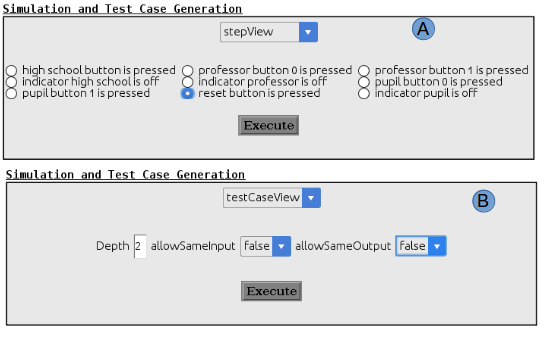
\includegraphics[width=.9\textwidth]{./images/Two_Views_Panel.png}
\caption{Simulation and test case generation panels, A) step-by-step simulation
view and B) test case generation view}
\label{fig:PanelView}
\vspace{-.2cm}
\end{figure*}
\vspace{-.2cm}
\subsubsection{Debugging Using Step-by-Step Simulation}
In order to debug quiz controller we previously generated we will perform a few
simulation steps: we first select the following inputs on the panel:
\emph{pupil Button 0} is set to \textsf{ON} and the remaining signals are set to
\textsf{OFF}.
The generated outputs reveal that the pupil indicator is in the \textsf{ON}
state which is the intended behavior. We then set the \emph{reset button
is pressed} to \textsf{ON} while the rest of the input signals are
set to \textsf{OFF}.
We expect that the controller's outputs are all set to the \textsf{OFF} state
in response to the reset, however the controller sets the indicator for the
pupil to the \textsf{ON} state as shown in Figure~\ref{fig:simError}. This investigation leads us to identify
an error in ``Req6'' of Figure~\ref{fig:QC_reqs}, where the pupil indicator is mistakenly turned on.
 \begin{figure*}[!h]
\centering
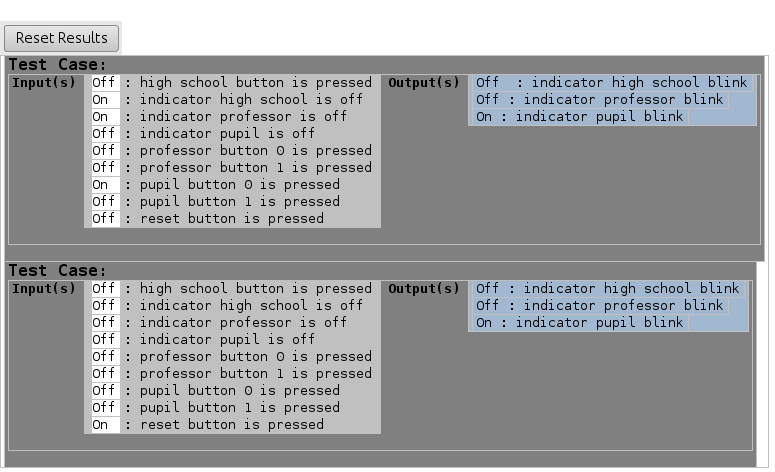
\includegraphics[width=1\textwidth]{./images/Simulation_Error.png}
\caption{Error identified during step-by-step simulation}
\label{fig:simError}
\vspace{-.6cm}
\end{figure*}
%\vspace{-.3cm}
\subsubsection{Automatic Test Cases Generation} 
\vspace{-.5cm}
Due to lack of space in this document, we are not able to present in a
screenshot a set results of test case generation for presentation at the
demonstration. However, during the demo we will exemplify our tool's test
generation capabilities by creating test set based on the available test generation parameters: test case length, repetition of
inputs in the test case allowed / not allowed and more than one sensor turned on
per input vector allowed / not allowed.

\section{Discussion}
Discussion will go here\ldots

\emph{Notes:} 
Point can be arised that if you are generating code from the model why do we need tests? we can sell our
idea by stating that we don't necessarly want to generate the code but write the
controller requirements as EARS and somebody else can write the code. Some
engineers don't rely on automatic code generation and want to develop/build
controllers explicitly. In such a situation, test case generation would help to
perform conformance between the specified controller and its respective implementation.
More points:
4. Code generation and synthesizer for EARS-based requirements
5. Test case generation for conformance checking of the generated controller
6. Interfacing with Matlab Simulink
5. Viewing the Results
7. Lessons learned
8. Start discussing the steps as flow model and follow exactly the same
steps!!!! 
8.1 Expression of Controller Requirements as EARS and related Models (e.g.,
Glossary) 
8.2 MPS constraints to ensure completeness of the EARS-based requirements
(hint: discuss some examples if something breaks) 
8.3 Test case generation process (step-by-step) that includes interfacing with
simulink, test case generation sequences, showing the results of the results as
inputs and output as the SimulinkResult model
\emph{Notes:}
Point can be arised that if you are generating code from the model why do we need tests? we can sell our
idea by stating that we don't necessarly want to generate the code but write the
controller requirements in EARS and somebody else can write the code. Some
engineers don't rely on automatic code generation and want to develop/build
controllers explicitly. In such a situation, test case generation would help to
perform conformance between the specified controller and its respective
implementation. 
dots
\emph{Notes:} 
Point can be arised that if you are generating code from the model why do we need tests? we can sell our
idea by stating that we don't necessarly want to generate the code but write the
controller requirements as EARS and somebody else can write the code. Some
engineers don't rely on automatic code generation and want to develop/build
controllers explicitly. In such a situation, test case generation would help to
perform conformance between the specified controller and its respective implementation.

\section*{Acknowledgements}
This work presented in this paper was developed in the context of the
``IETS3'' research project, funded by the German Federal Ministry of Education
and Research under code 01IS15037A/B.

\bibliographystyle{plain}
\bibliography{./bibliography}
\end{document}
